\chapter{Reading network interactions throughout development}

\epigraph{Development...}{Stanislas Dahaene}

\section{Motivation}



In the previous chapter, we established that reading does not appear to be "simply" a change in sensory systems. There are also more global changes in the degree of integration of different RSNs, especially those related to attention and executive control. However, this analysis was conducted in emerging readers: the participants were approximately 10 years old and were at a point in their education where basic skills were in place, but they were still relatively inexperienced readers.

It could be that the differences between the modalities were due to active support processes that were occuring between executive and attention regions, as the participants performed reading, a relatively novel task. On the one hand, advocates of a "parallel" model might assert that additional cognitive processes are used to "bootstrap" reading skill at early ages, so that differences between the two systems should decrease with maturity and reading experience as the two systems merge. On the other hand, the "parasitic" model of reading would predict that differences would persist, or even become exaggerated, as the two systems become more efficient for their respective tasks. In this chapter, then, we seek to replicate these results in a new cohort of subjects with a different set of passages, and then to investigate the effects of developmental maturity on the reorganizaton of brain networks during reading and listening.

There were two primary motivations in this study:

\begin{itemize}
	\item Which areas "converge" and "diverge" throughout development?
	\item What shifts in connectivity patterns do we see?
\end{itemize} 

\section{Methods}

\subsection{Participants}

To collect subjects at different stages in development, participants in this study were drawn from multiple study and age groups. They fell into three categories:

\begin{itemize}
	\item A group of children (ages 8 to 10) were selected from the third wave of the longitudinal study described in chapter 2. 
	\item A group of adolescents (ages 11 to 14) were selected. These participants were part of a large, cross-sectional study on the cognitive components of reading.
	\item A group of adults (ages 18 to 30) were selected, largely from a population of university research assistants and graduate students.
\end{itemize}

All subjects provided approval and were compensated according to our IRB.

\begin{table}[t]
	\renewcommand{\tabcolsep}{0.09cm}
	\centering
	\begin{tabular}{lc}
\toprule
Measure &               Value \\
\midrule
Subjects                        &              42 \\
Mean age                        &    10.51 (0.33) \\
Sex                             &      21 M, 23 F \\
WASI Full-Scale IQ, Vocabulary  &    52.91 (9.38) \\
Test of Word Reading Efficiency &  104.66 (18.07) \\
\bottomrule
\end{tabular}
	\caption{Participant demographics for study 2.}
	\label{table:ch4-participants}
\end{table}

\subsection{Functional MRI task design}

The task design for this study paralleled that of Chapter 2. Subjects were presented up to four separate runs of a passage comprehension task. The task included two passage blocks ("PASS"), two baseline attention blocks ("ATTN") and a trailing resting-state block ("REST"). Each task was performed in either the visual or auditory modality.

The contents of the passages differed from those of the tasks discussed in chapter 2, although they were also balanced to the same third-grade reading level using Coh-Metrix. 

\subsection{Data acquisition and processing}

Functional MRI data were acquired on a Philips Achieva 3T MR scanner under the previously described parameters. Data were pre-processed in FSL and the CONN Toolbox before being analyzed. See the Methods section of Chapter 2 for a detailed description of preprocessing routines and their parameters.

\subsection{Activation analyses}

We calculated subject-level contrast maps as described previously ("listening + reading vs. rest", "listening vs. reading"). At the group-level, we used age at scan as a continuous variable to estimate the effect of age on comprehensino-related activation and modality differences.

As before, we also investigated these effects in the connectome space as well 


\subsection{Connectivity analyses}
There was a high degree of similarity between the areas that were activated in reading and in listening, reflecting the common language core. Fig. \ref{fig:ch3-reading-connectome-activations} shows the activation statistics for each node, relative to rest, plotted against each other. There was a very high correlation coefficient ($r = 0.00$), reflecting the high degree of shared activity patterns between listening and reading.


% A scan run was included in the analysis only if a participant had both listening and reading scans in the same genre (e.g. auditory-expository and reading-expository). Therefore, for each year, a participant had data from either 2 or 4 scan runs (about 9 or 18 minutes of resting-state scan time, respectively). A scan session was excluded based on the following parameters: high-motion volumes exceeding 20 percent; poor task performance; and absence of a paired modality scan. In total, resting-state data from 50 children in the third wave (152 scans) and 45 children in the fourth wave (162 scans) met inclusion criteria. 

Attention and comprehension measures were not related to modality of stimulus presentation (see Fig. \ref{fig:ch3-task-performance}). There was a trend towards difference in median FDRMS between scan modalities (paired t-test, $t = 1.94$, $p = 0.059$), so we also replicated analyses with a stricter motion threshold (no more than 10 percent outliers in a scan run). The main results from analysis of this 35 subject (116 scan runs) cohort were broadly consistent.
\section{Results}

% \begin{figure}[t]
% 	\centering
%     \caption[Relationship between activation in visual word form area and age.]{}
% \end{figure}

Differences related to modality fell into three categories: sensory processing areas, including the insula, superior temporal gyrus, and secondary visual processing areas; and hetero-modal association areas, most notably the inferior frontal gyrus and angular gyrus; and somato-motor regions, including the premotor cortex and lateral geniculate nucleus of the thalamus (Fig. \ref{fig:ch3-modality-differences-attn}). Areas showing greater activation in listening were focused on primary auditory cortex and the dorsal attention network.

% \begin{figure}[t]
% 	\centering
%     \caption[Global participation coefficient as a function of age.]{}
% \end{figure}

\begin{figure}[t]
	\centering
	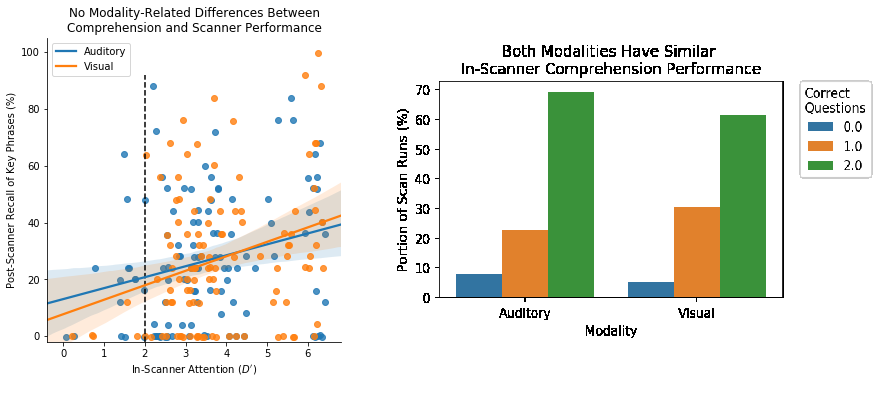
\includegraphics[height=3in]{ch3-task-performance}
    \caption[Behavioral metrics of passage performance were unrelated to modality.]{Both the in-scanner comprehension question and out-of-scanner recall questionnaire were unrelated to the modality of presentation.}
	\label{fig:ch3-task-performance}
\end{figure}

In the case of comprehension, we found that there was lower path length within modules during rest, while there were decreases in between-network connectivity during language.

For the modality contrast, One of the main takeaways is that there is greater access between auditory and other areas during reading -- this runs counter to our hypothesis that there would be less access to these areas. Visual areas, on the other hand, show less internal connectivity, reflecting the de-clustering of these areas during reading. 


% \begin{figure}[t]
% 	\centering
%     \caption[Similarity between reading and listening networks as a function of age.]{}
% \end{figure}


% \begin{figure}[t]
% 	\centering
%     \caption[]{}
% \end{figure}

\section{Discussion}

% Fronto-parietal description
% Task-based neuroimaging provides us with a rich description of the functions of frontoparietal network. The frontoparietal network is an assembly of brain regions encompassing the lateral frontal and parietal cortices along with insular, anterior/mid cingulate, and inferior temporal areas that have been broadly implicated in a variety of higher-level cognitive tasks \citep{Fedorenko2013}. Some have described the frontoparietal network as supporting active and adaptive online control, initiating and adjusting goal-directed mental systems \citep{Dosenbach2007}, while others have proposed a more general superordinate role in directing cognition \citep{Niendam2012}. The most obvious relationship of the frontoparietal network to language is its proximity to Broca’s area, known for its critical role in language articulation. Rather than thinking of this area (traditionally, Brodmann areas 44 and 45) as exclusively or primarily language-related, it has been argued that Broca’s area supports hierarchical executive processing, such as the segmentation (``chunking'') of auditory language and the flexible combination of words \citep{Koechlin2006}. Thus, while Broca's area plays a role in the unification of representations, prefrontal cortex (and the larger frontoparietal network) may play a higher-level control and initiating role in language and other processes \citep{Hagoort2005}. 

% Right hemisphere
% Our findings show that in stronger readers, the left frontoparietal RSN is expanded to include portions of the right posterior middle and superior temporal cortex.  These regions may play a number of roles in more skilled readers.  First, these right hemisphere regions are homologues of important left hemisphere language areas. The left posterior superior and middle temporal gyri are major secondary processing areas for written and auditory word stimuli \citep{Price2012}. In the right hemisphere, these areas are understood to play a complementary role, with a sensitivity to both emotional and prosodic elements \citep{Jung-Beeman2005}. Thus, the expansion of the frontoparietal network to these homologues could represent greater ``recruitment'' of complimentary language areas, facilitating  the integration of language-related information.  Secondly, these right hemisphere areas are subregions of the generally bilateral ventral attention RSN \citep{Yeo2011}.  Nonetheless in task-based studies, this network shows more of a right-sided bias \citep{Fox2006}.  As such, good readers may be better at integrating visual information with more high-order information.  These explanations need not be mutually exclusive.

% Ventral attention network
% While we found an expansion of the left frontoparietal RSN to regions of the ventral attention RSN in good readers, we did not find an association between variation in the ventral attention RSN itself and individual differences in reading ability. The ventral attention network detects salient or unexpected stimuli in the environment \citep{Vossel2014}. In this way the ventral attention network can act as a ‘circuit breaker’ for the dorsal system to help reorient attention \citep{Corbetta2002}. It may thus help orient individuals to new information from the visual environment (i.e. text) and, by coupling stimulus-driven attentional areas with the frontoparietal network, it may help construct updated mental representations of linguistic material. The leftward aspects of the ventral attention network underlie crucial reading-related areas, including occipito-temporal cortex, which performs orthographic processing, and temporo-parietal cortex, important for semantic binding \citep{Taylor2013}. The absence of reading-related variance associated with the entire bilateral RSN may reflect the diversity of functions that these areas serve in basic visual and auditory processing, as well as language and reading. 
